\section{Natural Clouds}
Clouds are a substantial part of Earth's weather. They provide shade from the glistening sun on hot days and reflect the heat at night, keeping the ground warmer.
For a layman, clouds are comprehensible and useful indicators for telling the weather. If they are dark and low-hanging, they bring rain. If they are puffy and scarce, they predict fair weather ahead.

\subsection{Types of Clouds}
In order to create a \gls{wrs} that is able to display many different cloudscapes, all distinct types of clouds have to be understood first.
Natural clouds are typically identified by two major factors: shape and \gls{altitude}.

\begin{figure}[H]
    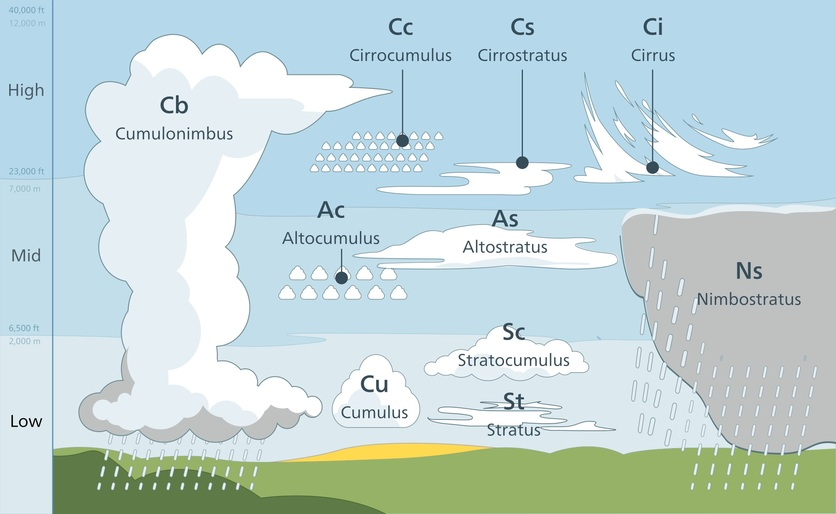
\includegraphics[width=\linewidth]{clouds-types.jpg}
    \captionof{figure}{Different categorizations of cloudshapes \protect\cite{cloudtypes}.}
    \label{img:ui:mockup:live}
\end{figure}

\noindent
This graphic from \emph{sciencelearn} provides and excellent overview of all distinct cloud types.
Each type is depicted in its signature shape and marked with the scientific name and abbreviation.
The \gls{altitude} is further split into three categories "low", "mid" and "high". 
